\chapter{Learned Relaying under Unknown and Mismatched Channels}\label{sec:unknown-channels}

This chapter tests learned relaying on selected channels with memory and model mismatch, following the matched memoryless controls of Chapter~\ref{sec:experiments}. The main comparison is with the implemented AF and zero-threshold DF baselines; matched sequence detection provides a stronger reference where the required channel information is supplied.

On the fixed three-tap BPSK channel, a 170-parameter windowed MLP substantially reduces destination BER relative to AF and zero-threshold DF. Those two mappings approach a $0.25$ high-SNR floor for the selected taps; the MLP's fixed-budget measurements continue to fall through 16~dB. This does not establish a limitation of all memoryless detectors, nor generalization to an unknown impairment family. The MLP is trained on this fixed filter. Later random-channel studies test unseen draws from a family represented during training.

No statistically resolved advantage over matched Viterbi MLSE is demonstrated in the BPSK comparison. Exact taps at inference and finite training samples are different information resources. MLSE minimizes sequence error, not BER; the QPSK BCJR control in Section~\ref{sec:bcjr-benchmark} measures bit errors at the relay output only. End-to-end BCJR performance is not measured. Cost comparisons are architecture- and implementation-specific: the small BPSK trellis is cheaper in nominal arithmetic than the MLP.

The following studies locate useful operating regimes for the tested learned relays, without claiming an exhaustive deployment map.

\paragraph{A conceptual ladder of assumptions.} Table~\ref{tbl:layers} organizes separate experiments by channel memory and available channel information. Modulation, fading, training, and evaluation budgets also differ between studies. The ladder is therefore an explanatory organization, not a controlled ablation that changes only one assumption at a time.

\begin{longtable}[]{@{}c>{\raggedright\arraybackslash}p{0.21\linewidth}>{\raggedright\arraybackslash}p{0.25\linewidth}>{\raggedright\arraybackslash}p{0.36\linewidth}@{}}
\caption[The four layers of the argument]{Four groups of experiments and representative measured outcomes. The rows organize the argument; they do not hold every experimental condition fixed. Classical entries identify the strongest implemented comparator in each group}\label{tbl:layers}\tabularnewline
\toprule\noalign{}
Layer & Assumptions & Strongest classical & Outcome \\
\midrule\noalign{}
\endfirsthead
\toprule\noalign{}
Layer & Assumptions & Strongest classical & Outcome \\
\midrule\noalign{}
\endhead
\bottomrule\noalign{}
\endlastfoot
1 & Memoryless, known channel, perfect CSI (Chapter~\ref{sec:experiments}) & Symbol-wise DF, zero trainable parameters & \textbf{Classical wins.} On the canonical QPSK/Rayleigh setup itself (Table~\ref{tbl:table2}), DF $0.1218$ against the MLP's $0.1229$ at 8~dB: the learned relay only matches DF, at 169 parameters against none (H2). \\
2 & \;+ channel memory (3-tap ISI), CSI still perfect (Section~\ref{sec:unknown-channel-experiment}) & Viterbi MLSE with exact taps & \textbf{Split.} The memoryless relays break outright, DF rising from $0.1802$ at 8~dB to $0.2457$ at 20~dB. The MLP restores the link ($0.0065$ at 8~dB), but genie-CSI Viterbi is ahead of it at every point where both are resolved: $0.001354$ against that $0.0065$ at 8~dB, and nominally below $3.0\times10^{-8}$ at 16~dB against the MLP's $1.20\times10^{-7}$. The advantage widens with SNR rather than holding at a fixed margin --- in required transmit power, $+0.26$~dB at a $10^{-1}$ target, $+1.18$ at $10^{-2}$, $+1.88$ at $10^{-3}$ and $+2.53$ at $10^{-4}$ (Table~\ref{tbl:tableE6}). The fixed filter is supplied exactly to the trellis and represented through finite training samples for the MLP; these information resources are not equivalent. \\
3 & \;+ CSI uncertainty: a finite pilot budget (Section~\ref{sec:partial-posterior}) & Pilot-aided LS estimate then MLSE & \textbf{Crossover.} At 10~dB, Viterbi-est holds $0.0283$ on 200 pilots and $0.0335$ on 20, both beating the pilot-free MLP's $0.0486$; by 10 pilots it has degraded to $0.0545$ and the MLP leads. The classical advantage is real but purchased with pilots. \\
4 & \;+ unseen realization from the trained family, redrawn per block (Sections~\ref{sec:composite-channel}, \ref{sec:blind-channel}) & CMA blind equalization & \textbf{Learned relay wins.} At 20~dB the MLP reaches $0.00262$ against CMA's $0.00329$, while decision-directed blind MLSE is unstable, non-monotonic and worse at 20~dB ($0.0498$) than at 16~dB ($0.0374$). The margin in BER is modest; the margin in stability and in per-block cost is not. \\
\end{longtable}

The comparator changes from a symbol-wise relay in the memoryless control to a sequence detector in the ISI study. Viterbi's sequence-ML guarantee applies to its specified channel likelihood, not to a mismatched estimated model. The learned relays instead use fixed weights trained on the specified impairment distribution.

The tested baselines are not exhaustive. Pilot-based and blind alternatives trade estimation effort and overhead against payload BER. The learned relay requires no test-time pilot estimate or online adaptation, but its training distribution remains part of its channel knowledge. Generalization outside that family is not established.

\paragraph{Relationship to the canonical model.} The canonical setup of this thesis (Chapter~\ref{sec:experiments}) assumes a memoryless two-hop relay channel with white noise, perfect receiver-side CSI, and uncoded transmission. The present chapter deliberately departs from those assumptions by introducing impairments that are not part of the canonical model, including channel memory (3-tap intersymbol interference), amplifier nonlinearity, unknown phase, and channel-model mismatch. Consequently, sequence-detection and equalization techniques such as Viterbi MLSE, pilot-aided channel estimation, and blind equalization become relevant only in this chapter. The goal is not to replace the canonical study, but to evaluate whether the conclusions established under matched memoryless conditions remain valid when the underlying channel model no longer represents the true channel.

\begin{figure}[htbp] \noindent \makebox[\textwidth][l]{%
\begin{tikzpicture}[ >=latex, node distance=2.3cm, block/.style={rectangle, draw, thick, minimum width=2.0cm, minimum height=1.0cm, align=center}, imp/.style={rectangle, draw, very thick, fill=black!6, minimum width=2.4cm, minimum height=1.1cm, align=center}, relayblock/.style={rectangle, draw, very thick, dashed, minimum width=2.0cm, minimum height=1.1cm, align=center} ]
\node[block] (S) {Source\\BPSK};
\node[imp, right=2.0cm of S] (C) {Unknown Hop-1\\ISI $\times$ PA $\times$ phase};
\node[relayblock, right=2.0cm of C] (R) {Relay\\$f_\theta(\cdot)$}; \node[block, right=2.0cm of R] (D) {Destination\\Decision};
\draw[->,thick] (S) -- (C);
\draw[->,thick] (C) -- node[above,align=center]{\footnotesize unknown\\[-2pt]\footnotesize to relay} (R);
\draw[->,thick] (R) -- node[above,align=center]{Hop 2\\$h_2[i],n_2[i]$} (D);
\node[below=0.9cm of C, align=center, font=\footnotesize] (note) {Departure from the canonical model:\\ channel \emph{memory} (3-tap ISI), nonlinearity, unknown phase.\\ Noise remains white; only the \emph{channel} violates memorylessness.};
\draw[dotted] (C.south) -- (note.north);
\end{tikzpicture}%
} \caption[Unknown and mismatched-channel study]{Schematic of the composite impairment study. Hop 1 includes memory, amplifier nonlinearity, and block phase; Hop 2 is compensated Rayleigh fading with AWGN. The learned relay is trained on the impairment family, while the pilot-aided classical baseline estimates a linear channel. Individual studies use the configurations stated in their methods}
\label{fig:ext-unknown}
\end{figure}

\section{Layer 1 --- Matched Memoryless Channel: The Control}\label{sec:layer-one}

The matched memoryless comparison is reported in Sections~\ref{sec:siso-bpsk-performance-baseline-relay-comparison} and~\ref{sec:minimum-relay-size}. It provides a reference setting, not a causal isolation of the reasons for performance differences in later, differently configured studies.

\section{Layer 2 --- Channel Memory with Perfect CSI: Classical Failure and Learned Mitigation}\label{sec:unknown-channel-experiment}

\textbf{Goal:} Test whether the learned relay's value changes qualitatively when the channel violates the assumptions under which AF and DF are (near-)optimal: do the \emph{memoryless} classical relays fail on an unknown channel while the minimal $170$-parameter MLP mitigates by learning it from data (H5)?

Unlike the canonical experiments, where each transmitted symbol can be processed independently, the 3-tap ISI channel couples adjacent symbols in time. The sufficient statistic for detection is therefore no longer a single received sample, making sequence detection the relevant classical benchmark. To make the classical side as strong as possible, the study benchmarks against the optimal sequence detector: Viterbi MLSE applied to the 3-tap FIR/ISI channel \cite{Forney1972MLSE} with genie CSI, and a practical variant with a 200-pilot least-squares estimate.

MLSE is introduced here solely because the channel now contains memory. In the canonical memoryless setting of Chapter~\ref{sec:experiments}, per-symbol detection is sufficient and sequence detection provides no additional benefit. The need for MLSE therefore arises from the deliberate introduction of ISI in this chapter rather than from the system model studied elsewhere in the thesis.

\paragraph{Relation to data-driven detection.} Learning channel-dependent detector computations is established prior work: ViterbiNet \cite{Shlezinger2020ViterbiNet} combines learned likelihoods with a Viterbi recursion. The present contribution is a comparison of small feedforward relays and the specified classical baselines under the particular channel, pilot, and computation budgets reported here.

The flat-channel controls, pilot-budget sweep, and blind comparison delimit that empirical claim. They do not establish that prior work lacks such boundary studies, or that three taps become unidentifiable at five pilots. The pilot results concern estimation quality in the tested finite-sample systems.

\paragraph{\textbf{Trials.}}
\begin{itemize}
 \item \textbf{Topology:} SISO (both hops)
    \item \textbf{Modulation:} BPSK (DBPSK for the unknown-phase control and the composite cascade)
    \item \textbf{Hop-1 channel (unknown to all relays); Hop-2 (equal SNR per hop):}
    \begin{itemize}
        \item 3-tap ISI, $h=[1.0,0.7,0.5]/\lVert h\rVert$ (Hop 2: AWGN)
        \item Flat unknown channels (phase, gain, asymmetry; Section~\ref{sec:flat-unknown-channels}) (Hop 2: Rayleigh)
        \item Composite cascade of ISI, amplifier nonlinearity, and unknown phase (Section~\ref{sec:composite-channel}) (Hop 2: Rayleigh)
    \end{itemize}
    \item \textbf{Relays:}
    \begin{itemize}
        \item AF
        \item Symbol-wise DF
        \item MLP (window 11, one hidden layer of 13 tanh units, 170 parameters; trained at SNR $\in\{5,10,15\}$ dB using the canonical training protocol)
        \item For ISI setups only: Viterbi MLSE applied to the 3-tap FIR/ISI channel, evaluated with either genie CSI or a 3-tap least-squares channel estimate obtained from 200 pilot symbols
    \end{itemize}
\item \textbf{Evaluation:} 10 trials $\times$ 100{,}000 bits per SNR point, SNR range 0--20 dB. To rule out the influence of the particular random initialization and training data used to fit the MLP, the network is retrained independently with three different random seeds, giving 30 BER samples per cell (3 training instances $\times$ 10 inference trials). The mean is their average. The confidence interval is \emph{not}: the ten trials inside one seed share a trained network, so they resample Monte Carlo noise but not training variance and are not 30 independent draws from the population the claim concerns. Intervals are therefore computed hierarchically --- average within each seed, then a Student-$t$ interval on the three seed means, $t_{2,0.975} = 4.303$ rather than $1.96$, deliberately wide because three points say little about a spread. Pooling all 30 as i.i.d.\ divides by $\sqrt{30}$ where the effective sample size is nearer 3; on the MLP rows here that understates the interval by a factor of about seven to eight (at 8~dB on S1, ${\pm}1.3\times10^{-3}$ against a pooled ${\pm}1.8\times10^{-4}$). AF and DF are barely affected, as expected, since neither has a trained network to vary across seeds.
\end{itemize}

The ISI channel admits a sharp analytic prediction, and it is not confined to the asymptote. With BPSK symbols i.i.d.\ and equiprobable, the relay observes $y[n] = h_0 x[n] + h_1 x[n-1] + h_2 x[n-2] + v[n]$ and a memoryless slicer returns $\operatorname{sign}(y[n])$. Conditioned on $x[n]=+1$ the two interfering symbols take one of $2^{2}=4$ equiprobable sign patterns, each fixing an effective amplitude $A(s_1,s_2) = h_0 + s_1 h_1 + s_2 h_2$, so
\begin{equation}\label{eq:slicer-floor}
P_e(\gamma) \;=\; \tfrac{1}{4}\!\!\sum_{s_1,s_2 \in \{\pm 1\}}\!\! \Phi\!\left(\frac{-A(s_1,s_2)}{\sigma}\right),
\qquad \sigma^{2} = \frac{1}{2\gamma},\quad \gamma = 10^{\mathrm{SNR_{dB}}/10}.
\end{equation}
For $h = [1.0, 0.7, 0.5]$ normalized the four amplitudes are $1.6678$, $0.9097$, $0.6065$ and $-0.1516$. As $\sigma \to 0$ each term tends to $0$ where $A>0$ and to $1$ where $A<0$, so the limit is the fraction of interference patterns that \emph{flip the symbol sign} --- here exactly one of four, giving the floor of $0.25$, approached from below.

AF reaches the same floor, but this needs its own argument rather than an appeal to inheritance, since AF performs no hard decision. The relay forwards $g(A + n_1)$ with $g$ the power-normalization gain and the destination slices $g(A + n_1) + n_2$; a positive scale cannot change a sign, so the effective statistic is $A + n_1 + n_2/g$. That is the same four-amplitude structure with an inflated variance $\sigma^{2}(1 + g^{-2})$, $g^{2} = 1/(\mathbb{E}[A^{2}] + \sigma^{2})$, so the $\sigma \to 0$ limit is again the fraction of sign-flipping patterns. The floor belongs to the four amplitudes, not to the decision rule. The two relays approach it differently, and AF is the better of the two at high SNR \emph{because} of its extra noise: on the one pattern whose amplitude is negative, DF errs with probability tending to one, while AF's additional noise still occasionally rescues the decision.

Both closed forms predict the measured curves across the sweep, not the asymptote alone. The measured rows below are the S1 columns of the same three-seed run that produces Table~\ref{tbl:tableE6}, read at six of its eleven SNR points rather than the four that table tabulates (\texttt{isi\_slicer\_floor.py} for the closed forms, \texttt{e6\_sim\_ported.py} for the measurements):

\begin{center}\small
\begin{tabular}{lrrrrrr}
\toprule
SNR (dB) & 6 & 8 & 12 & 16 & 18 & 20 \\
\midrule
DF closed form, Eq.~\eqref{eq:slicer-floor} & $0.1786$ & $0.1803$ & $0.2009$ & $0.2280$ & $0.2389$ & $0.2460$ \\
DF measured & $0.1802$ & $0.1802$ & $0.2009$ & $0.2296$ & $0.2391$ & $0.2457$ \\
AF closed form & $0.1939$ & $0.1814$ & $0.1835$ & $0.2075$ & $0.2213$ & $0.2338$ \\
AF measured & $0.1943$ & $0.1813$ & $0.1834$ & $0.2067$ & $0.2213$ & $0.2349$ \\
\bottomrule
\end{tabular}
\end{center}

\noindent The closed forms reproduce the broad high-SNR trend and the different minima of AF and DF. The DF expression is a relay-slicer calculation and omits second-hop errors; the AF expression includes both hops with an ensemble power-normalization approximation. Differences of order $10^{-3}$ in the displayed values preclude claiming agreement to three or four decimal places. This analytic check does not validate the stopping rule or confidence coverage of the historical rare-event simulations.

The $0.25$ limit is specific to the chosen taps and zero-threshold rule. In general, average $\mathbf{1}\{A<0\}+\tfrac12\mathbf{1}\{A=0\}$ over the four equiprobable interference patterns; zero-amplitude ties contribute one half. If $h_0>|h_1|+|h_2|$, this floor is zero. For the selected taps, the noiseless observations conditioned on the current bit form disjoint sets, even though one amplitude has the opposite sign. A non-monotonic symbol-wise MAP rule could exploit those sets. The result therefore demonstrates a benefit over the evaluated AF and zero-threshold DF mappings, not an impossibility theorem for all memoryless detectors.

\subsection{Control: Flat (Memoryless) Unknown Channels}\label{sec:flat-unknown-channels}

Before attributing any classical failure to ``unknownness,'' it must be separated from \emph{memory}. This subsection isolates unknown channels that are \emph{flat} (memoryless): the receiver chain does not know the channel parameters, but the channel introduces no intersymbol coupling. Three physically motivated cases are tested, each with the parameter redrawn per block and unknown to all relays: (F1) an unknown carrier phase $\theta\sim\mathcal{U}[0,2\pi)$ (oscillator/synchronization offset), with a DBPSK source and conventional differential detection as the classical relay; (F2) an unknown positive gain $g\sim\mathcal{U}[0.3,2.0]$ (path loss / AGC error), coherent BPSK; and (F3) an unknown per-branch amplitude asymmetry $a_+\!\neq\!a_-$ (per-symbol saturating-PA gain), coherent BPSK. The learned relay is trained identically to before. Its size differs slightly by setup, because the phase case consumes complex I/Q pairs ($22$ inputs into $7$ hidden units, $169$ parameters) while the two real-valued cases take an $11$-sample window into $13$ ($170$); the two are the same architecture class at the same budget, and are labelled by their exact counts in the table.

These flat-channel controls preserve sample-wise channel mappings, although the differential receiver uses adjacent samples. They test three specified forms of parameter uncertainty; they do not cover all unknown memoryless channels.

\textbf{Conclusion.} In these three controls, the MLP and classical relay have similar measured BER: the largest difference is $0.0012$ across the tabulated points and $0.0064$ across the full sweep. Differential detection accommodates the block phase, and a positive gain preserves the noiseless BPSK sign. These observations show that the tested uncertainty alone need not defeat the chosen classical receiver; they do not prove equivalence or exclude benefits on other flat-channel families.

\begin{longtable}[]{@{}lllll@{}}
\caption[Flat unknown channels]{Flat-channel controls at 8/12/16/20~dB. Learned-relay means use three training seeds and ten inference trials per seed. Similar measured BER is not a statistical equivalence claim. MLP-169 uses complex I/Q input; MLP-170 uses real input}\label{tbl:tableE6flat}\tabularnewline
\toprule\noalign{}
Flat channel & Relay & 8 dB & 12 dB & 16/20 dB \\
\midrule\noalign{}
\endfirsthead
\toprule\noalign{}
Flat channel & Relay & 8 dB & 12 dB & 16/20 dB \\
\midrule\noalign{}
\endhead
\bottomrule\noalign{}
\endlastfoot
Unknown phase (DBPSK) & DF (diff.) & 0.0654 & 0.0286 & 0.0121 / 0.0050 \\
 & MLP-169 & 0.0666 & 0.0286 & 0.0121 / 0.0050 \\
Unknown gain & DF & 0.0739 & 0.0298 & 0.0122 / 0.0050 \\
 & MLP-170 & 0.0739 & 0.0300 & 0.0122 / 0.0050 \\
Branch asymmetry & DF & 0.0669 & 0.0286 & 0.0121 / 0.0050 \\
 & MLP-170 & 0.0671 & 0.0287 & 0.0121 / 0.0050 \\
\end{longtable}

\textbf{Conclusion (H5, within the tested scope).} The fixed-filter BPSK study shows a large MLP improvement over AF and zero-threshold DF. Matched Viterbi gives lower measured BER over the resolved comparison range: at 8~dB the genie and 200-pilot LS values are $0.001354$ and $0.001460$, respectively, versus $0.0065$ for the MLP. There is no 8-dB crossover in the corrected data. At 0~dB the MLP and genie means are close and the study does not resolve their ordering. Interpolated required-SNR penalties relative to genie MLSE vary with the target: $0.26$, $1.18$, $1.88$, and $2.53$~dB at BER $10^{-1}$ through $10^{-4}$. They are not a universal $1$--$1.5$~dB offset. The fixed-budget checkpoint results support the separation through 16~dB, not an extrapolation beyond that range.

\textbf{Note on simulation validity.}
The observed AF/DF rise is specific to the evaluated relay mappings and tap vector; it is not a theorem about every memoryless relay or every ISI channel. The fixed-budget measurements at 12, 14, and 16~dB support a large MLP improvement over those memoryless comparators. The historical 18--20~dB entries use exposure determined by the first error and are retained only as exploratory records. They do not establish the precise BER, a confidence bound valid under correlated errors, or monotonicity beyond the fixed-budget points; separately declared fixed-budget reruns are required before making those claims.

\textbf{Status of the rare-event estimates.} Extending the exposure to $10N_1$ after the first error does not produce an ordinary fixed-budget estimate. The historical 16~dB entry (16 errors in 334{,}002{,}040 bits) is retained only in the provenance record; it is replaced here by a predeclared fixed-budget confirmation: three independently trained checkpoints, each evaluated over $10^8$ bits in 1000 blocks. This run records 36 MLP errors in $3\times10^8$ bits and yields a mean BER of $1.20\times10^{-7}$; the wide across-checkpoint interval is descriptive rather than an i.i.d.-bit confidence claim. The 12 and 14~dB points likewise use three predeclared $10^7$-bit runs. The historical 18--20~dB values remain exploratory, are omitted from the MLP curve in Figure~\ref{fig:figE6}, and must not support precision or monotonicity claims pending the same validation.

\begin{longtable}[]{@{}p{3.1cm}p{2.5cm}p{2.5cm}p{2.5cm}p{2.5cm}@{}}
\caption[Unknown-channel BER (fixed-budget validation through 16~dB)]{Destination BER for fixed three-tap BPSK ISI followed by AWGN. At 8~dB, AF/DF/MLP use the original three-seed study; the Viterbi rows use the matched-protocol run. AF/DF/MLP at 12 and 16~dB use respectively 10M and 100M bits per checkpoint (three checkpoints). Viterbi entries with $<$ are nominal independent-Bernoulli rule-of-three bounds from zero observed errors: 1M bits at 12~dB, 100M at 16 and 20~dB. They indicate insufficient data to estimate a positive BER, not zero true BER; correlated-error coverage is not established}\label{tbl:tableE6}\tabularnewline
\toprule\noalign{}
Relay & 8 dB & 12 dB & 16 dB & 20 dB \\
\midrule\noalign{}
\endfirsthead
\toprule\noalign{}
Relay & 8 dB & 12 dB & 16 dB & 20 dB \\
\midrule\noalign{}
\endhead
\bottomrule\noalign{}
\endlastfoot
AF & 0.1813 & 0.1835 & 0.2075 & 0.2349 \\
DF & 0.1802 & 0.2009 & 0.2280 & 0.2457 \\
\textbf{MLP (170p)} & \textbf{0.0065} & \textbf{$1.456\times10^{-4}$} & \textbf{$1.20\times10^{-7}{}^\dagger$} & not validated \\
Viterbi (genie CSI) & 0.001354 & $<3.0\times10^{-6}$ & $<3.0\times10^{-8}$ & $<3.0\times10^{-8}$ \\
Viterbi (200-pilot LS) & 0.001460 & $<3.0\times10^{-6}$ & $<3.0\times10^{-8}$ & $<3.0\times10^{-8}$ \\
\multicolumn{5}{p{0.94\linewidth}}{\footnotesize $^\dagger$ At 16~dB: 36 MLP errors in 300M bits. The 14-dB fixed-budget mean is $9.2\times10^{-6}$. Historical adaptive 18--20~dB MLP estimates are excluded from quantitative conclusions.} \\
\end{longtable}

\begin{figure}[htbp]
\centering
\pandocbounded{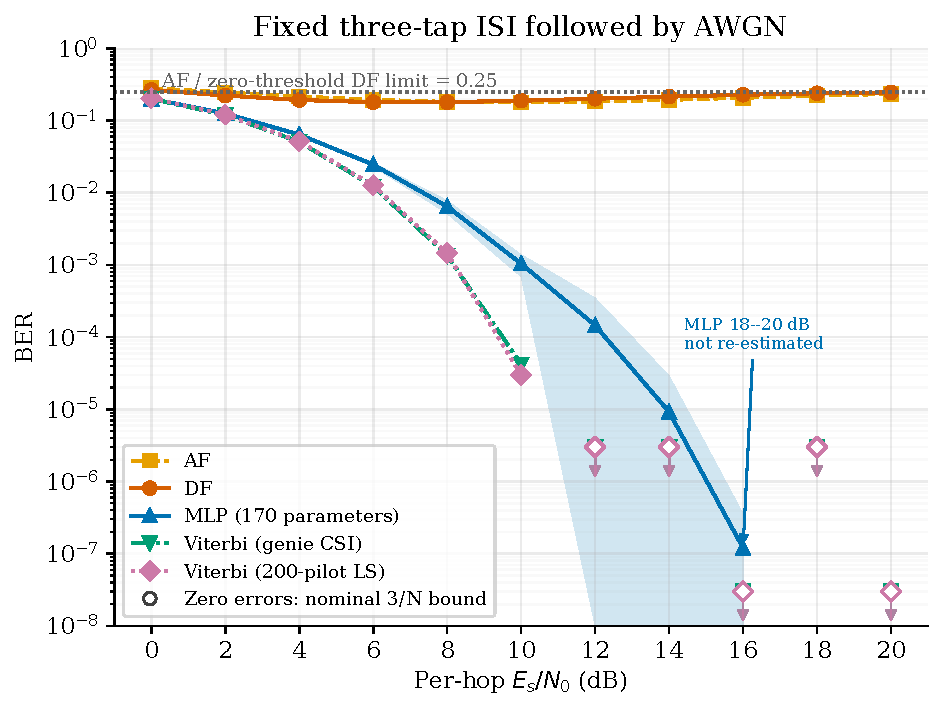
\includegraphics[width=\linewidth,height=0.39\textheight,keepaspectratio]{results/e6_unknown_channel.pdf}}
\caption[Unknown-channel relaying, fixed-budget validation through 16~dB]{Destination BER versus per-hop $E_s/N_0$. The original figure is regenerated with the same matched Viterbi sources as Table~\ref{tbl:tableE6}. MLP points above 16~dB are omitted. Open Viterbi markers show zero-error nominal $3/N$ bounds at the actual bit budgets, with downward arrows; these are not measured BERs. AF/DF/MLP bands use the stored across-checkpoint uncertainty at 12--16~dB and the historical intervals below 12~dB}\label{fig:figE6}
\end{figure}

\subsection{Does the Result Generalize to QPSK?}\label{sec:qpsk-unknown-channel}

The unknown-ISI study above uses BPSK throughout. The canonical setup of Chapter~\ref{sec:experiments} is QPSK, so this subsection asks whether the failure mode survives the move to that constellation. It is not a clean constellation control and is not offered as one: as Eq.~\eqref{eq:qpsk-hop1} below records, the QPSK study also puts an independent per-symbol fade on top of the fixed filter, so the two studies differ in channel as well as in modulation. Isolating the constellation would need a plain-QPSK-ISI run, which was not performed. The $0.25$ floor derived in Section~\ref{sec:unknown-channel-experiment} is a property of the \emph{binary zero-threshold} slicer: it counts the $2^{2}=4$ equiprobable interfering-symbol patterns that flip a $\pm1$ decision. It does not imply a QPSK symbol-error floor or a fixed QPSK BER, because QPSK decisions use two axes and this experiment also changes the fading model. The QPSK result is therefore a separate measured extension, not a direct theorem-level generalization. This subsection repeats the relay comparison with Gray-coded QPSK in place of BPSK, using the same nominal per-hop SNR axis ($\gamma=10^{\text{SNR}_{\text{dB}}/10}$) and the same relay families generalized to the complex alphabet: AF, symbol-wise DF (hard per-axis decision), a $193$-parameter $4$-class MLP-QPSK classifier (window 11, softmax cross-entropy, trained at SNR $\in\{5,10,15\}$ dB), and Viterbi MLSE generalized to the complex QPSK trellis ($4^{2}=16$ states, complex branch metrics).

One difference from the BPSK study matters more than it first appears. Hop~1 here is not the plain ISI channel of Section~\ref{sec:unknown-channel-experiment} but
\begin{equation}\label{eq:qpsk-hop1}
y[n] \;=\; g[n]\,(h * x)[n] \;+\; v[n], \qquad g[n] = |\,\mathcal{CN}(0,1)\,|\ \text{i.i.d.},
\end{equation}
an independent Rayleigh magnitude on every symbol on top of the fixed filter. A trellis built from $h$ alone is therefore \emph{not} a genie-CSI detector on this channel: its branch metrics compare $y[n]$ against unfaded expected values, leaving a residual $A^{2}(g[n]-1)^{2}$ that does not shrink as the noise does. Both detectors are reported below --- the taps-only trellis, and a genie-CSI trellis given $g[n]$ as well as $h$, which scales each branch's expected observation accordingly. Evaluation uses $10$ trials $\times$ $100{,}000$ bits per SNR point over the same $0$--$20$ dB range. No closed-form floor is derived for QPSK, so the curves below are reported as measured, not fit to a predicted asymptote. Because the QPSK relays are applied jointly to the complex signal rather than decomposed into two independent BPSK problems, and the per-relay power normalization is computed on total (I+Q) power, the resulting AF/DF operating points are not required to, and empirically do not, numerically match the BPSK figures of Table~\ref{tbl:tableE6} at the same SNR label; no such match is claimed.

\begin{longtable}[]{@{}llllll@{}}
\caption[QPSK unknown-channel BER (mean over 10 trials)]{QPSK unknown-channel BER (mean over 10 trials) on the per-symbol faded ISI channel of Eq.~\eqref{eq:qpsk-hop1}. AF and DF plateau at an elevated, non-monotonic BER across the SNR range tabulated, and the 193-parameter MLP-QPSK restores monotonically decreasing BER. The last two rows are the same trellis given different information: with the taps alone it is model-mismatched here and the MLP passes it above about 2~dB; given the per-symbol fading gains as well, it is the genie-CSI detector for this channel and leads the MLP everywhere.}\label{tbl:tableE6qpsk}\tabularnewline
\toprule\noalign{}
Setup & Relay & 8 dB & 12 dB & 16 dB & 20 dB \\
\midrule\noalign{}
\endfirsthead
\toprule\noalign{}
Setup & Relay & 8 dB & 12 dB & 16 dB & 20 dB \\
\midrule\noalign{}
\endhead
\bottomrule\noalign{}
\endlastfoot
QPSK: ISI $\to$ AWGN & AF & 0.2447 & 0.2116 & 0.2019 & 0.2100 \\
 & DF & 0.2197 & 0.2024 & 0.2074 & 0.2211 \\
 & \textbf{MLP-QPSK (193p)} & \textbf{0.1292} & \textbf{0.0827} & \textbf{0.0601} & \textbf{0.0508} \\
 & Viterbi (taps only) & 0.1307 & 0.0852 & 0.0670 & 0.0618 \\
 & \textbf{Viterbi (genie CSI)} & \textbf{0.0739} & \textbf{0.0155} & \textbf{0.0018} & \textbf{0.0001} \\
\end{longtable}

\begin{figure}[htbp]
\centering
\pandocbounded{\includegraphics[width=\linewidth,height=0.24\textheight,keepaspectratio]{results/unkchan_qpsk.png}}
\caption[QPSK unknown-channel relaying]{QPSK unknown-channel relaying, BER vs.\ SNR (10 trials, 100{,}000 bits/point). As with BPSK, AF and DF plateau far above the MLP and Viterbi curves. The MLP-QPSK curve separates below the \emph{taps-only} trellis beyond about 2 dB, but the correctly informed genie-CSI trellis (given the per-symbol fading gains as well as the taps) leads the MLP at every SNR, by a gap that widens with SNR}\label{fig:figE6qpsk}
\end{figure}

\textbf{Conclusion (QPSK with ISI and additional fading):} The evaluated QPSK experiment changes both the modulation and the channel, adding per-symbol Rayleigh magnitudes to the fixed ISI filter. Its results establish a benefit over the evaluated memoryless relays under that combined change. A plain-QPSK-ISI control with consistent $E_b/N_0$ accounting is required to isolate modulation order.

Two trellis detectors have to be distinguished on this channel, and Eq.~\eqref{eq:qpsk-hop1} is why. A trellis built from $h$ alone, on a channel that also fades per symbol, is model-mismatched rather than genie-informed, and its error rate flattens for that reason. Three controls on the same trellis (\texttt{qpsk\_trellis\_controls.py}, run under the exact configuration of Table~\ref{tbl:tableE6qpsk}) separate the two explanations at 20~dB: given the taps on the faded channel it reaches a symbol error rate of $0.113$; on the same channel with the fading removed, $0.000$; and given the fading gains as well, $0.0003$. The trellis is not at fault (it is verified never to return a path less likely than the transmitted sequence, and to reduce exactly to the nearest-symbol slicer when the ISI is removed) only its channel model was.

With the genie-CSI detector, the rounded destination BERs range from $0.3300$ against the MLP's $0.3389$ at 0~dB to $0.0001$ against $0.0508$ at 20~dB. The measured ordering agrees with the BPSK study, but the simultaneous modulation and channel changes prevent attributing that agreement to either factor alone.

The ordering is not an artefact of the error criterion either. A decomposition of the QPSK error events (\texttt{qpsk\_error\_decomposition.py}) separates the detectors on symbols as well as on bits: measured against the taps-only detector, the MLP is ahead on \emph{symbol} error rate as well from about 8~dB up ($0.0939$ against $0.1126$ at 20~dB), and the two lose almost the same number of bits per symbol error ($1.073$ against $1.090$), so the Gray map is not the route either. It cannot be, for a structural reason stronger than that measurement. The taps are real and the fading gain is a real magnitude, so $y[n] = g[n](h*x)[n] + v[n]$ separates into two independent real ISI channels carrying the in-phase and quadrature bits; conditional on the genie-supplied gains and taps, the symbol posterior therefore factorises into its I/Q bit marginals, and bit-wise MAP and symbol-MAP are the same detector on this channel, not merely close ones (\texttt{tests/test\_bcjr\_qpsk.py}, agreement to $5.6\times10^{-16}$).

At QPSK, the supplied-taps-and-gains Viterbi receiver substantially outperforms the 193-parameter MLP: the rounded destination BERs at 20~dB are $0.0001$ and $0.0508$. A precise multiplicative ratio should not be inferred from the rounded classical value. The supported benefit is relative to the tested memoryless baselines, not near-optimal BER. The relay-output BCJR control below addresses a different measurement endpoint.

\subsection{Relay-Output Control: BCJR/APP Against Viterbi MLSE}\label{sec:bcjr-benchmark}

Viterbi MLSE minimizes sequence error, whereas bit-MAP decisions minimize expected bit error under the supplied model \cite{BahlCockeJelinekRaviv1974BCJR}. The control in \texttt{qpsk\_bcjr\_benchmark.py} compares these two decisions with both taps and per-symbol fading gains supplied. It measures errors \emph{at the relay output before Hop~2}; Table~\ref{tbl:tableE6qpsk} measures destination errors. Thus this is not an end-to-end BCJR-versus-MLP experiment.

Two controls check the detector implementation. Removing fading while retaining ISI does not require MLSE and bit-MAP to agree: at 8~dB their BERs are $0.021764$ and $0.021424$, with paired difference $+0.00034\pm0.00016$, a resolved difference at the reported level. At 20~dB both record zero errors in $10^6$ bits; $3.0\times10^{-6}$ is a nominal independent-bit reference bound, not a proof of zero BER. Removing ISI is the appropriate exact-agreement control: BCJR reduces to the per-axis slicer on all $10{,}000$ tested symbols.

\begin{table}[htbp]
\centering
\caption[BER-optimal benchmark against Viterbi MLSE]{Genie-CSI Viterbi MLSE against the BER-optimal BCJR/APP detector on the same trellis, relay output, 10 trials of 100{,}000 bits. The interval is on the paired per-trial difference, $t(9,0.975)=2.262$}\label{tbl:bcjr-benchmark}
\begin{tabular}{rrrrl}
\toprule
SNR (dB) & Viterbi BER & BCJR BER & Relative gain & Paired 95\% CI \\
\midrule
0  & 0.250177 & 0.239113 & 4.42\% & resolved \\
4  & 0.162702 & 0.155861 & 4.20\% & resolved \\
8  & 0.068918 & 0.067245 & 2.43\% & resolved \\
12 & 0.015075 & 0.014857 & 1.45\% & resolved \\
16 & 0.001726 & 0.001725 & 0.06\% & includes zero \\
20 & 0.000127 & 0.000126 & 0.79\% & includes zero \\
\bottomrule
\end{tabular}
\end{table}

\textbf{Conclusion.} BCJR has no higher empirical relay-output BER at the sampled points; its paired advantage is not resolved at 16 and 20~dB. Bit-MAP optimality concerns expected loss under the model and does not guarantee ordering in every finite Monte Carlo sample. These controls support the local detector implementation. They neither establish an end-to-end BCJR margin against the MLP nor close the unmeasured BPSK bit-MAP comparison.

\subsection{A Fixed Composite Channel: Learned and Estimated-Model Relays}\label{sec:composite-channel}

This study cascades fixed three-tap ISI, a fixed saturating amplifier, and a randomly drawn block phase before additive noise, using DBPSK. It tests a combined impairment, not a factorial isolation of each cause. The implemented comparators are AF, differential detection, and pilot-LS Viterbi followed by differential decoding. The latter estimates a linear FIR model and is mismatched to the nonlinear amplifier; no claim that it is the strongest possible classical receiver is made. The 169- and 1{,}153-parameter MLPs are trained on this cascade family without receiving its analytic parameters at inference.

Evaluation uses 10 unique trials of 100{,}000 source bits per SNR and three trained MLP instances. Repeated classical seeds and the training/trial hierarchy prevent interpreting the historical plotting bands as independent-trial 95\% confidence intervals. They are retained only as descriptive bands. During this review, the composite AF path was found to add half the intended complex Hop~2 noise power. Its curve was rerun with the corrected variance, original ten unique trial seeds and bit budgets, recording errors, exposures and Student-$t$ intervals in \url{e6_unknown_channel_results/codex_composite_af_validation.json}. The other relays emit real signals and do not use the affected complex-noise branch; their stored point estimates are unchanged. Overlapping bands do not establish equivalence.

\textbf{Conclusion within this cascade.} AF and differential detection remain near BER $0.25$ at high SNR; this is an observation, not a derived universal floor for nonlinear channels. The 169-parameter MLP has much lower measured BER, reaching $2.5\times10^{-3}$ at 20 dB. Pilot-LS Viterbi has lower BER at 8~dB ($0.0674$ vs.\ $0.1073$ at 8 dB) and both round to $0.0025$ at 20 dB. Equal rounded values do not establish equivalent reliability. The larger MLP is also close at the last point, ending at a rounded $0.0025$ at 20 dB. Its mid-SNR means are lower than the small MLP's ($0.1016$ versus $0.1073$ at 8~dB; $0.0482$ versus $0.0542$ at 10~dB), but the historical intervals do not support a formal capacity-equivalence or paired-significance conclusion. These results support learned processing on this trained cascade family, not arbitrary impairment stacks, unseen channel families, or superiority over an optimally matched receiver.

\begin{figure}[htbp]
\centering
\pandocbounded{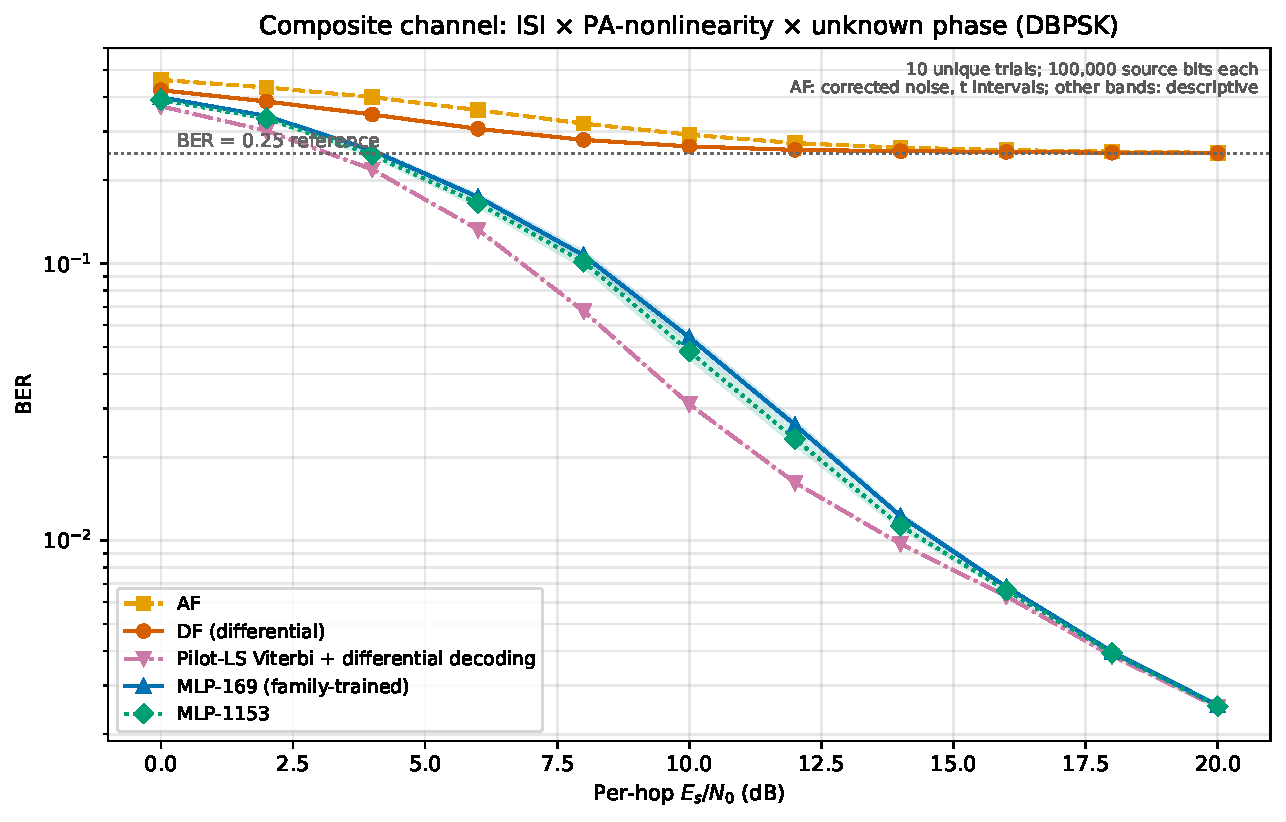
\includegraphics[width=\linewidth,height=0.36\textheight,keepaspectratio]{results/e6_composite.pdf}}
\caption[Composite multi-impairment channel]{Fixed ISI and amplifier with random block phase, DBPSK. The corrected AF curve uses ten unique fixed-budget trials and Student-$t$ intervals. Other curves retain historical point estimates and descriptive bands, which are not calibrated equivalence tests. Both MLPs were trained on this cascade family. Similar high-SNR rounded values do not demonstrate equal BER}\label{fig:figE6comp}
\end{figure}

\section{Layer 3 --- CSI Uncertainty: The Pilot-Budget Crossover}\label{sec:partial-posterior}

This is layer~3 of the ladder in Table~\ref{tbl:layers}: the pilot count is varied within the specified random composite-channel protocol. This differs from the preceding fixed-composite experiment. The pilot-aided trellis estimates a linear channel; it is not an oracle for the nonlinear cascade. Here channel information is limited: the pilot budget is finite, and the classical receiver must work from a correspondingly noisy estimate. Sweeping the pilot count on the composite channel at a fixed 10 dB operating point locates where the pilot-aided classical receiver ceases to beat the pilot-free learned relay, whose fixed trained estimator provides a horizontal reference (it uses no pilots at test). Its channel knowledge is amortized into its weights during training rather than estimated per block; the network is a discriminative estimator trained on the family, and its outputs have not been checked for calibration. \textbf{Evaluation:} 50 trials $\times$ 20{,}000 bits per operating point ($1{,}000{,}000$ bits), matching Section~\ref{sec:blind-channel} and for the same reason: the channel is redrawn per block, so trials are draws from the impairment family. In panel~(b) each trial is further subdivided into independent blocks of the swept length, so every block length is measured over the same total bit budget and over many channel draws rather than a single one.

\textbf{Conclusion (an estimation-variance cliff at 10 dB, and a rate--reliability tradeoff):} With a generous budget the classical partial posterior wins, as expected: pilot-aided Viterbi reaches payload BER $0.0285$ at 800 pilots and degrades only gently down to $0.0335$ at 20 pilots, comfortably below the MLP's pilot-free $0.0486$. At 10 pilots Viterbi has lost its edge, $0.0545$ against the MLP's $0.0486$, and at 5 pilots it reaches $0.1235$, because MLSE is then running on a badly estimated channel. The mechanism is estimation variance rather than rank deficiency: with 5 pilot observations and 3 complex taps the least-squares problem is formally overdetermined, but there are too few observations to average down the noise. The 95\% interval at that point is $0.1235 \pm 0.0304$, against $\pm 0.0011$ at 50 pilots. The MLP remains at $0.0486$ because it requires no per-block pilots after training on the channel family. Thus, at the measured 10-dB operating point, the crossover lies between 20 and 10 pilots. Its location is necessarily SNR-dependent because least-squares estimation error depends on noise power; no pilot-count sweep was run at another SNR, so a universal crossover is not claimed. The ordering is stable across the three trained MLP instances.

The practical force of this depends on block length, because a fixed pilot \emph{count} is a growing pilot \emph{fraction} as blocks shorten. Panel (b) sweeps block length at the same operating point with the classical receiver spending its minimum viable ten pilots per block, and adds blind CMA as the second pilot-free reference. The payload-BER confidence intervals overlap at the evaluated block lengths, both estimates being approximately $0.049$; the study has not established equivalence. At a 1000-symbol block the ten pilots cost $1\%$ of the block, whereas at a 40-symbol block, representative of low-latency or fast-varying links, they cost $25\%$, so the classical receiver carries data on only $75\%$ of the block against the learned relay's $100\%$ with no payload-BER difference detected at this budget.

Among the tested pilot-free methods, the fixed MLP has lower BER on these short blocks than CMA: CMA records $0.1723$ at $L=40$ and $0.1653$ at $L=1000$, versus its $0.0645$ long-block reference. This is consistent with limited adaptation time, but convergence failure is not isolated from other algorithmic settings. The MLP and pilot-aided receiver have no resolved difference at this budget; that is not proof of equal reliability. The conclusion is limited to the implemented baselines and block lengths.

\begin{figure}[htbp]
\centering
\begin{minipage}[t]{0.49\linewidth}\centering
  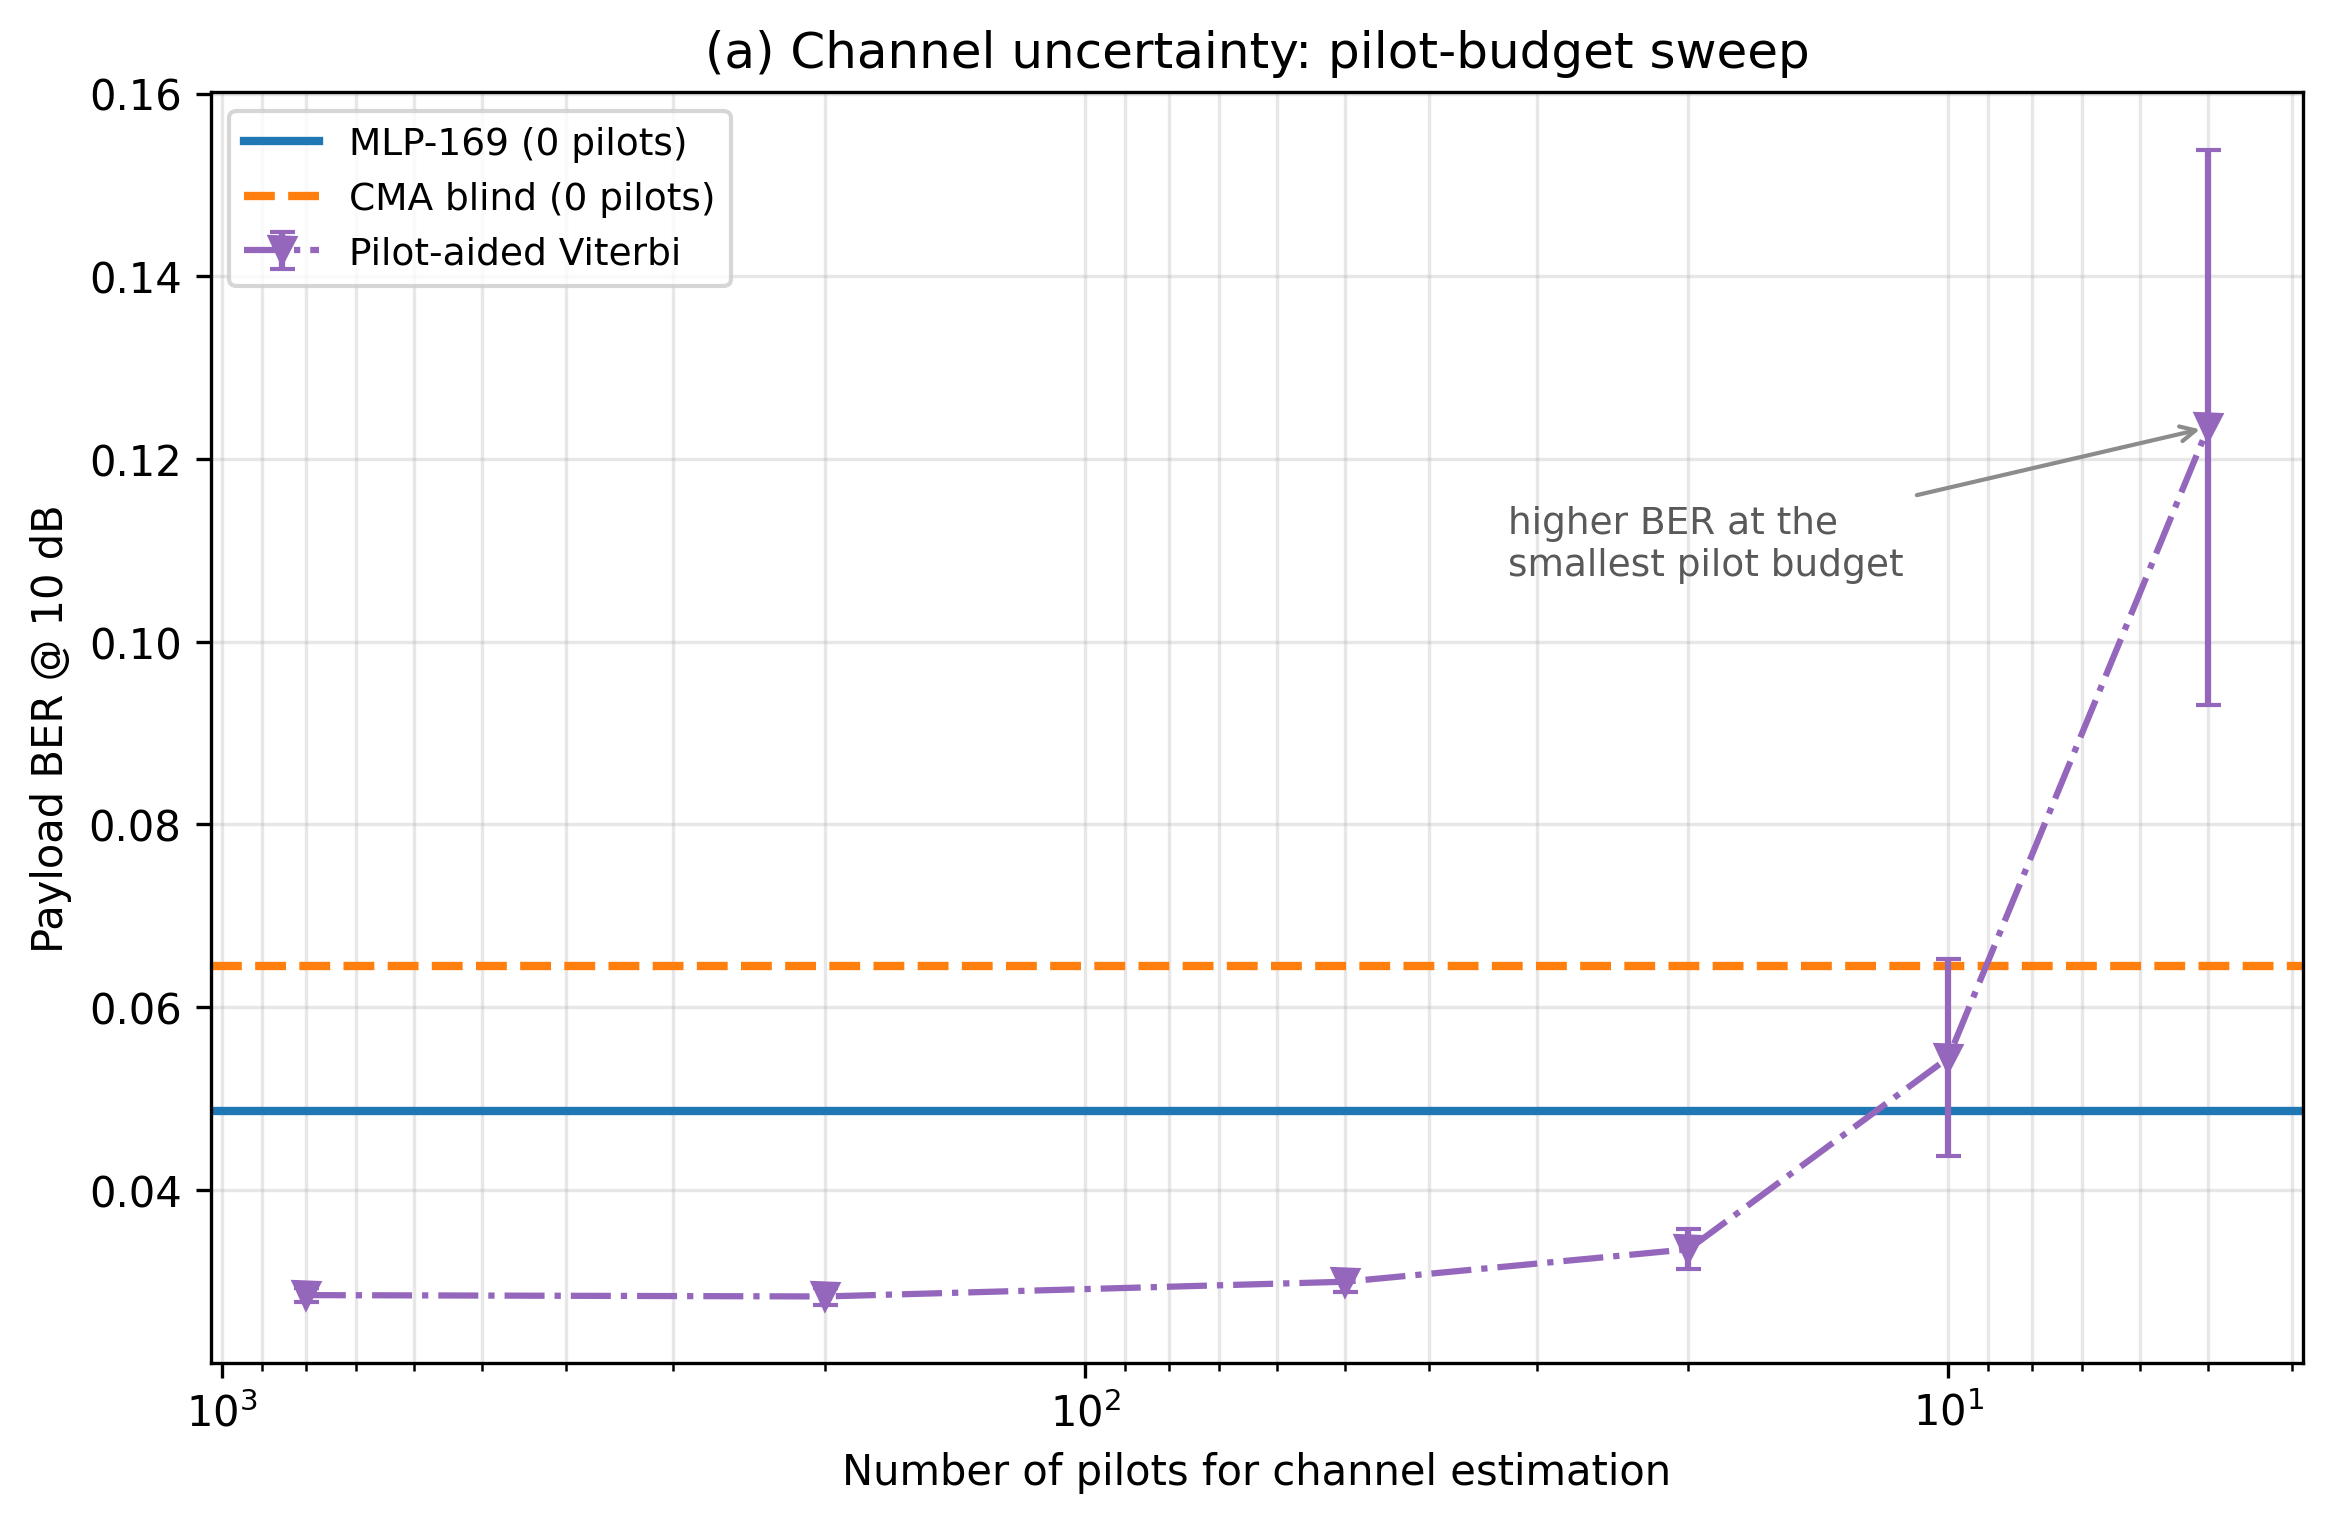
\includegraphics[width=\linewidth]{results/e6_partial_pilot_budget_sweep.png}\\[2pt]
  {\small (a) pilot-budget sweep at 10~dB}
\end{minipage}\hfill
\begin{minipage}[t]{0.49\linewidth}\centering
  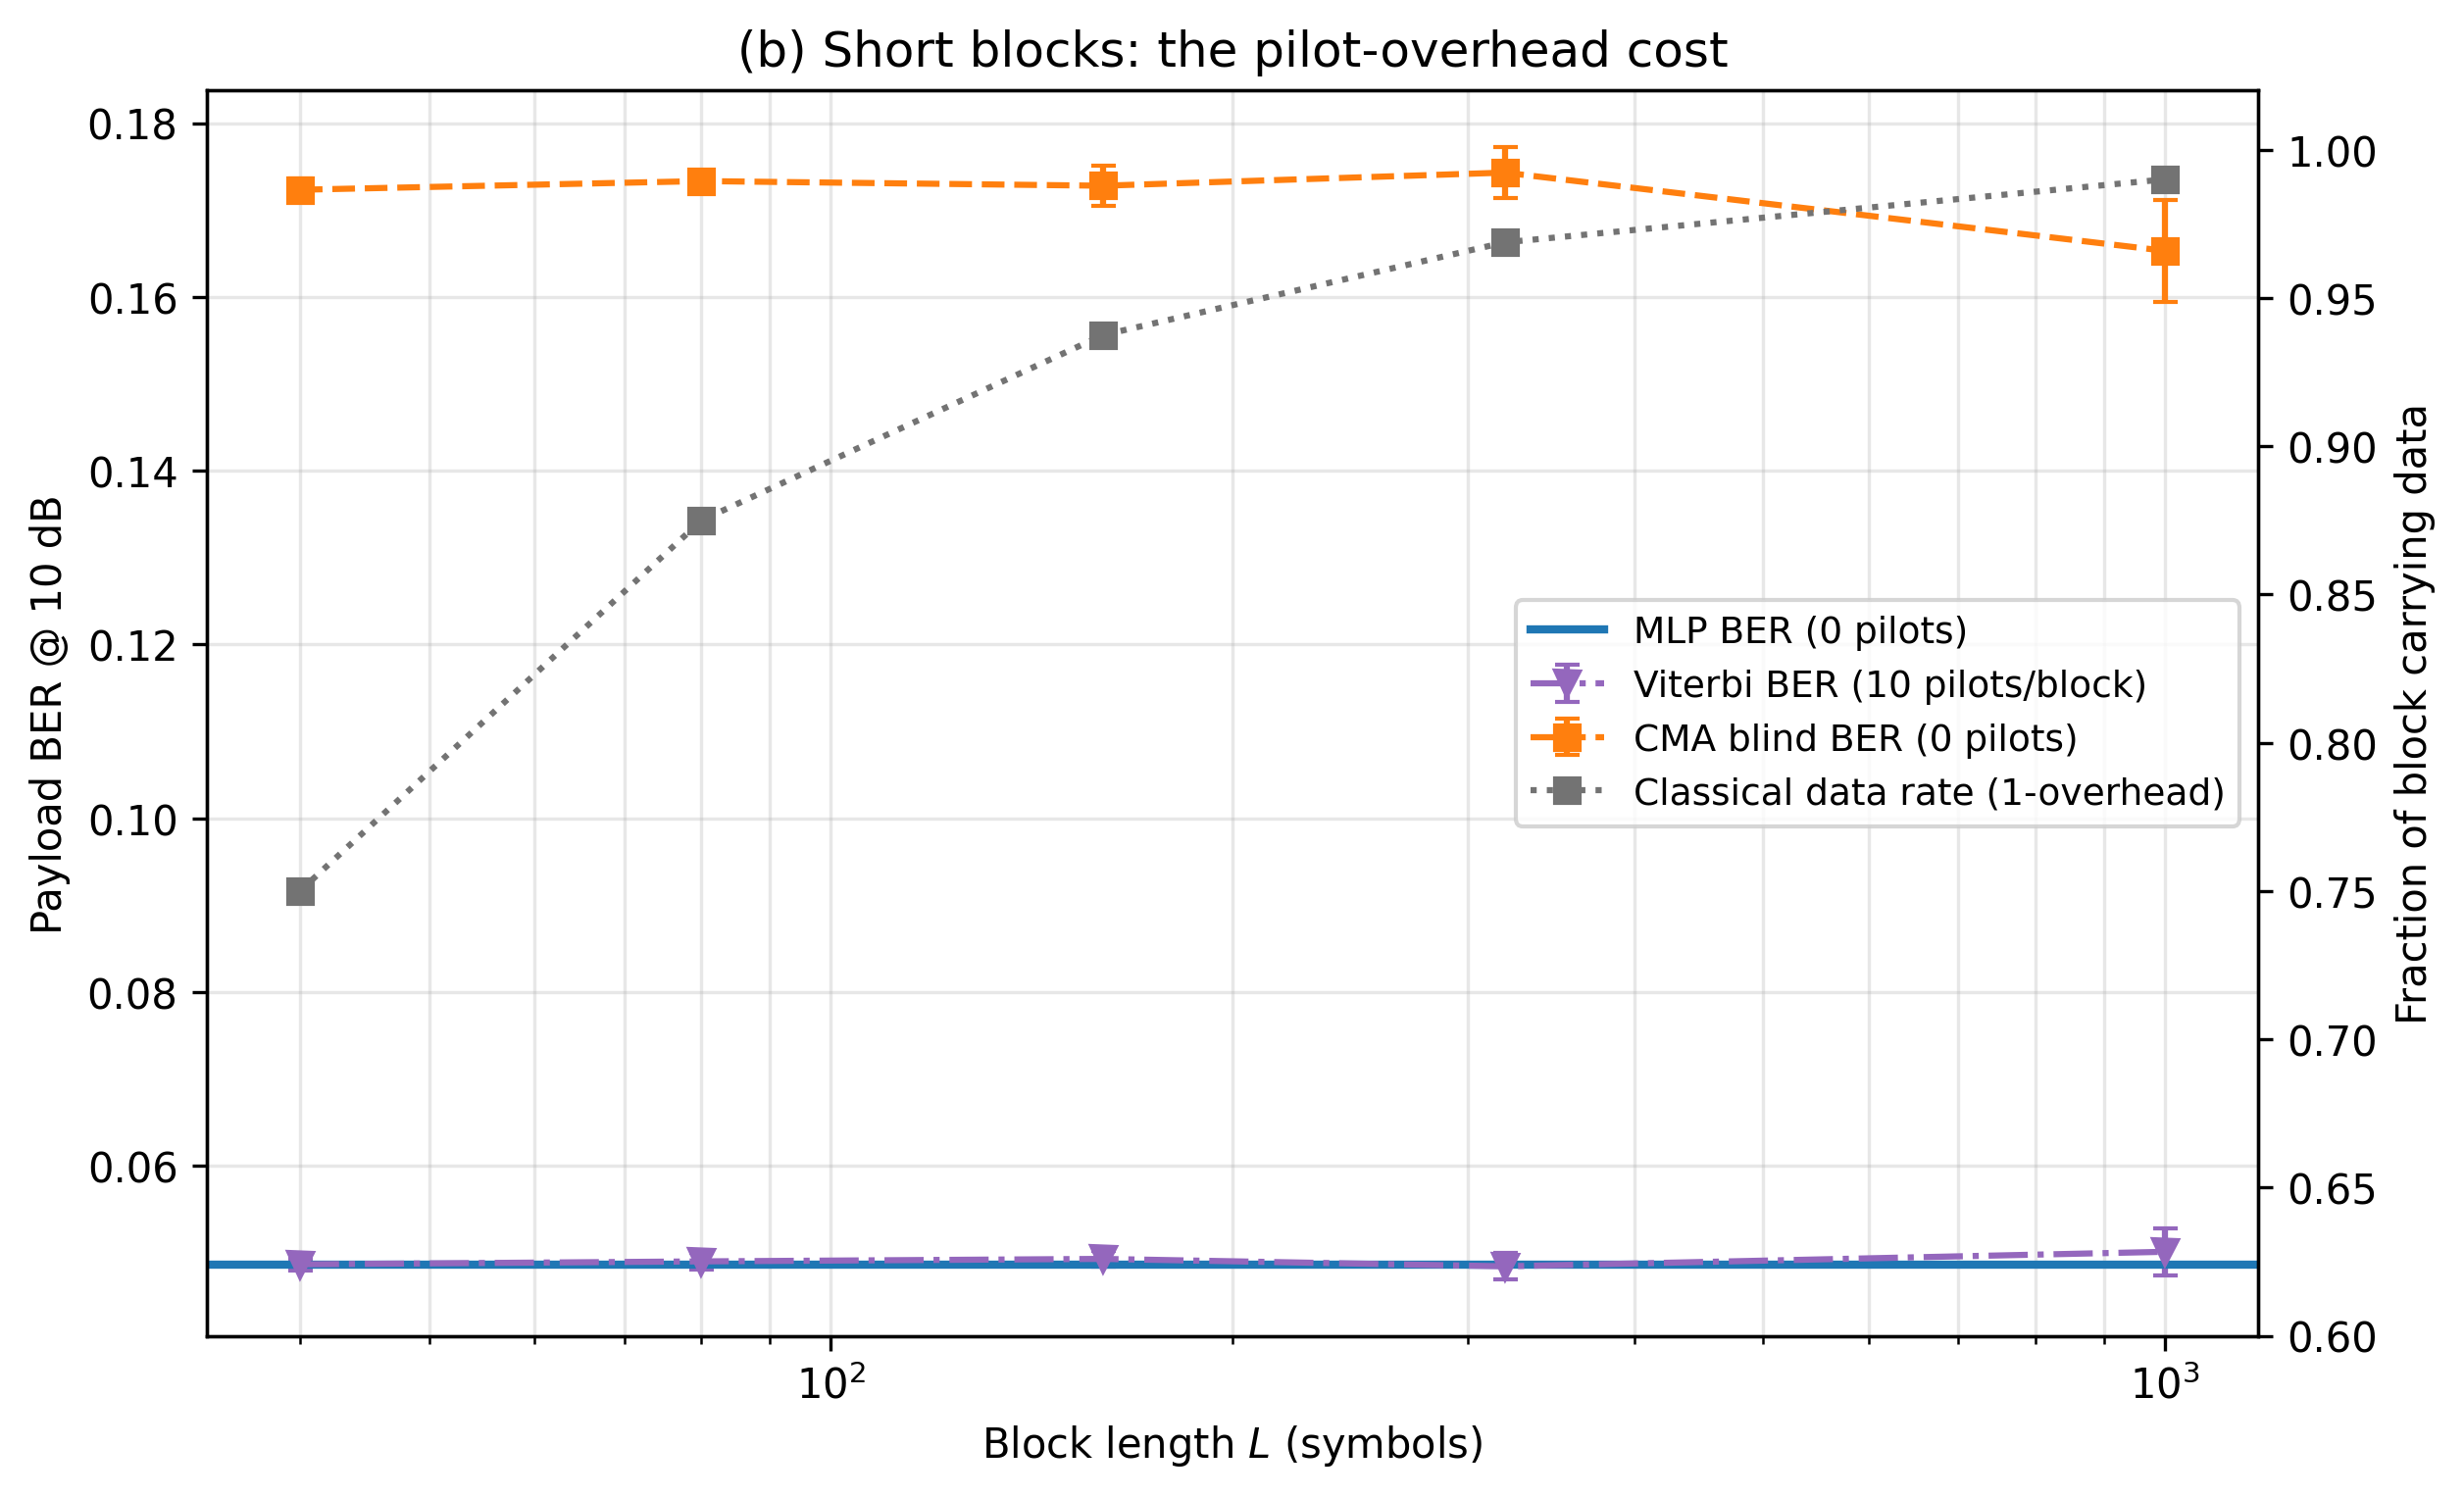
\includegraphics[width=\linewidth]{results/e6_partial_short_blocks_overhead.png}\\[2pt]
  {\small (b) block-length sweep at 10 pilots}
\end{minipage}
\caption[Finite-pilot sweeps: pilot budget and block length]{Finite-pilot regime; both panels are means over 50 channel draws at 20{,}000 bits/point. \textbf{(a)} Pilot-aided Viterbi outperforms the pilot-free MLP down to approximately 20 pilots per block, loses its edge by 10 pilots, and collapses at 5 pilots when the least-squares estimate becomes too noisy to construct a reliable trellis ($0.1235 \pm 0.0304$); the MLP is flat across the sweep, operating with a family-trained discriminative estimator and requiring no pilots. \textbf{(b)} With 10 pilots per block, pilot-aided Viterbi and the MLP have no detected payload-BER difference at the evaluated block lengths (both $\approx 0.049$), but the classical receiver's pilot overhead grows from approximately 1\% at $L=1000$ to 25\% at $L=40$. The tested CMA implementation has higher BER throughout. The MLP uses no pilots and has no resolved BER difference from the pilot-aided receiver at this budget; equivalence and superiority to untested pilot-free methods are not established}
\label{fig:e6_partial_pilot_budget}
\end{figure}

\section{Layer 4 --- Unknown Per-Block Realization: The Blind Regime}\label{sec:blind-channel}

This is layer~4, the bottom of the ladder. Per-block CSI and pilots are removed, and a fresh realization is drawn from the same impairment family used during MLP training. The comparison is against CMA, which assumes constant modulus and adapts an equalizer from the received block, and decision-directed MLSE, which bootstraps a channel estimate from its own decisions. Thus no method receives per-block CSI, but neither is assumption-free: the MLP knows the training distribution and CMA knows signal/equalizer structure. \textbf{Evaluation:} 50 independent channel draws $\times$ 20{,}000 bits per SNR point. Classical-method intervals use those 50 draws; neural uncertainty is assessed across trained instances rather than by treating repeated inference under one network as independent training evidence.

\paragraph{A correction to the blind equalizer.} The earlier fixed-step CMA implementation overflowed on longer blocks. The evaluated version normalizes its update by input-segment energy to limit this numerical instability. This is an implementation choice, not a proof that normalized CMA always converges or universally improves on fixed-step CMA. The results below concern the corrected implementation and its stated settings.

\textbf{Conclusion (learning narrowly leads CMA and avoids per-block adaptation):} The corrected CMA reaches BER $3.3\times10^{-3}$ at 20 dB, and the family-trained MLP reaches $2.6\times10^{-3}$. The MLP holds a small measured margin over the evaluated range, the MLP at $0.0955$ against CMA's $0.1182$ at 8 dB, while decision-directed blind MLSE is non-monotonic ($0.0374$ at 16 dB and $0.0498$ at 20 dB). Whether that margin is resolved is a question the intervals have to answer rather than the point estimates: the decision-directed MLSE interval at 8 dB is $\pm0.0201$, against the MLP's $\pm0.0026$ and CMA's $\pm0.0078$. This does not make CMA unstable: the observed instability belongs to the decision-directed MLSE implementation. CMA instead carries an online adaptation cost and requires enough samples to converge, whereas the MLP uses one fixed forward pass after offline training. For uncertainty reporting, the three trained MLP instances must be treated hierarchically rather than pooling their inference trials; classical methods have no training seed, so their effective sample size is the 50 independent channel draws. The supported conclusion is therefore narrow: on unseen per-block realizations from its training family, the MLP slightly outperforms the evaluated CMA implementation while avoiding per-block adaptation, and it avoids the non-monotonic behavior of the evaluated decision-directed MLSE.

\begin{figure}[htbp]
\centering
\pandocbounded{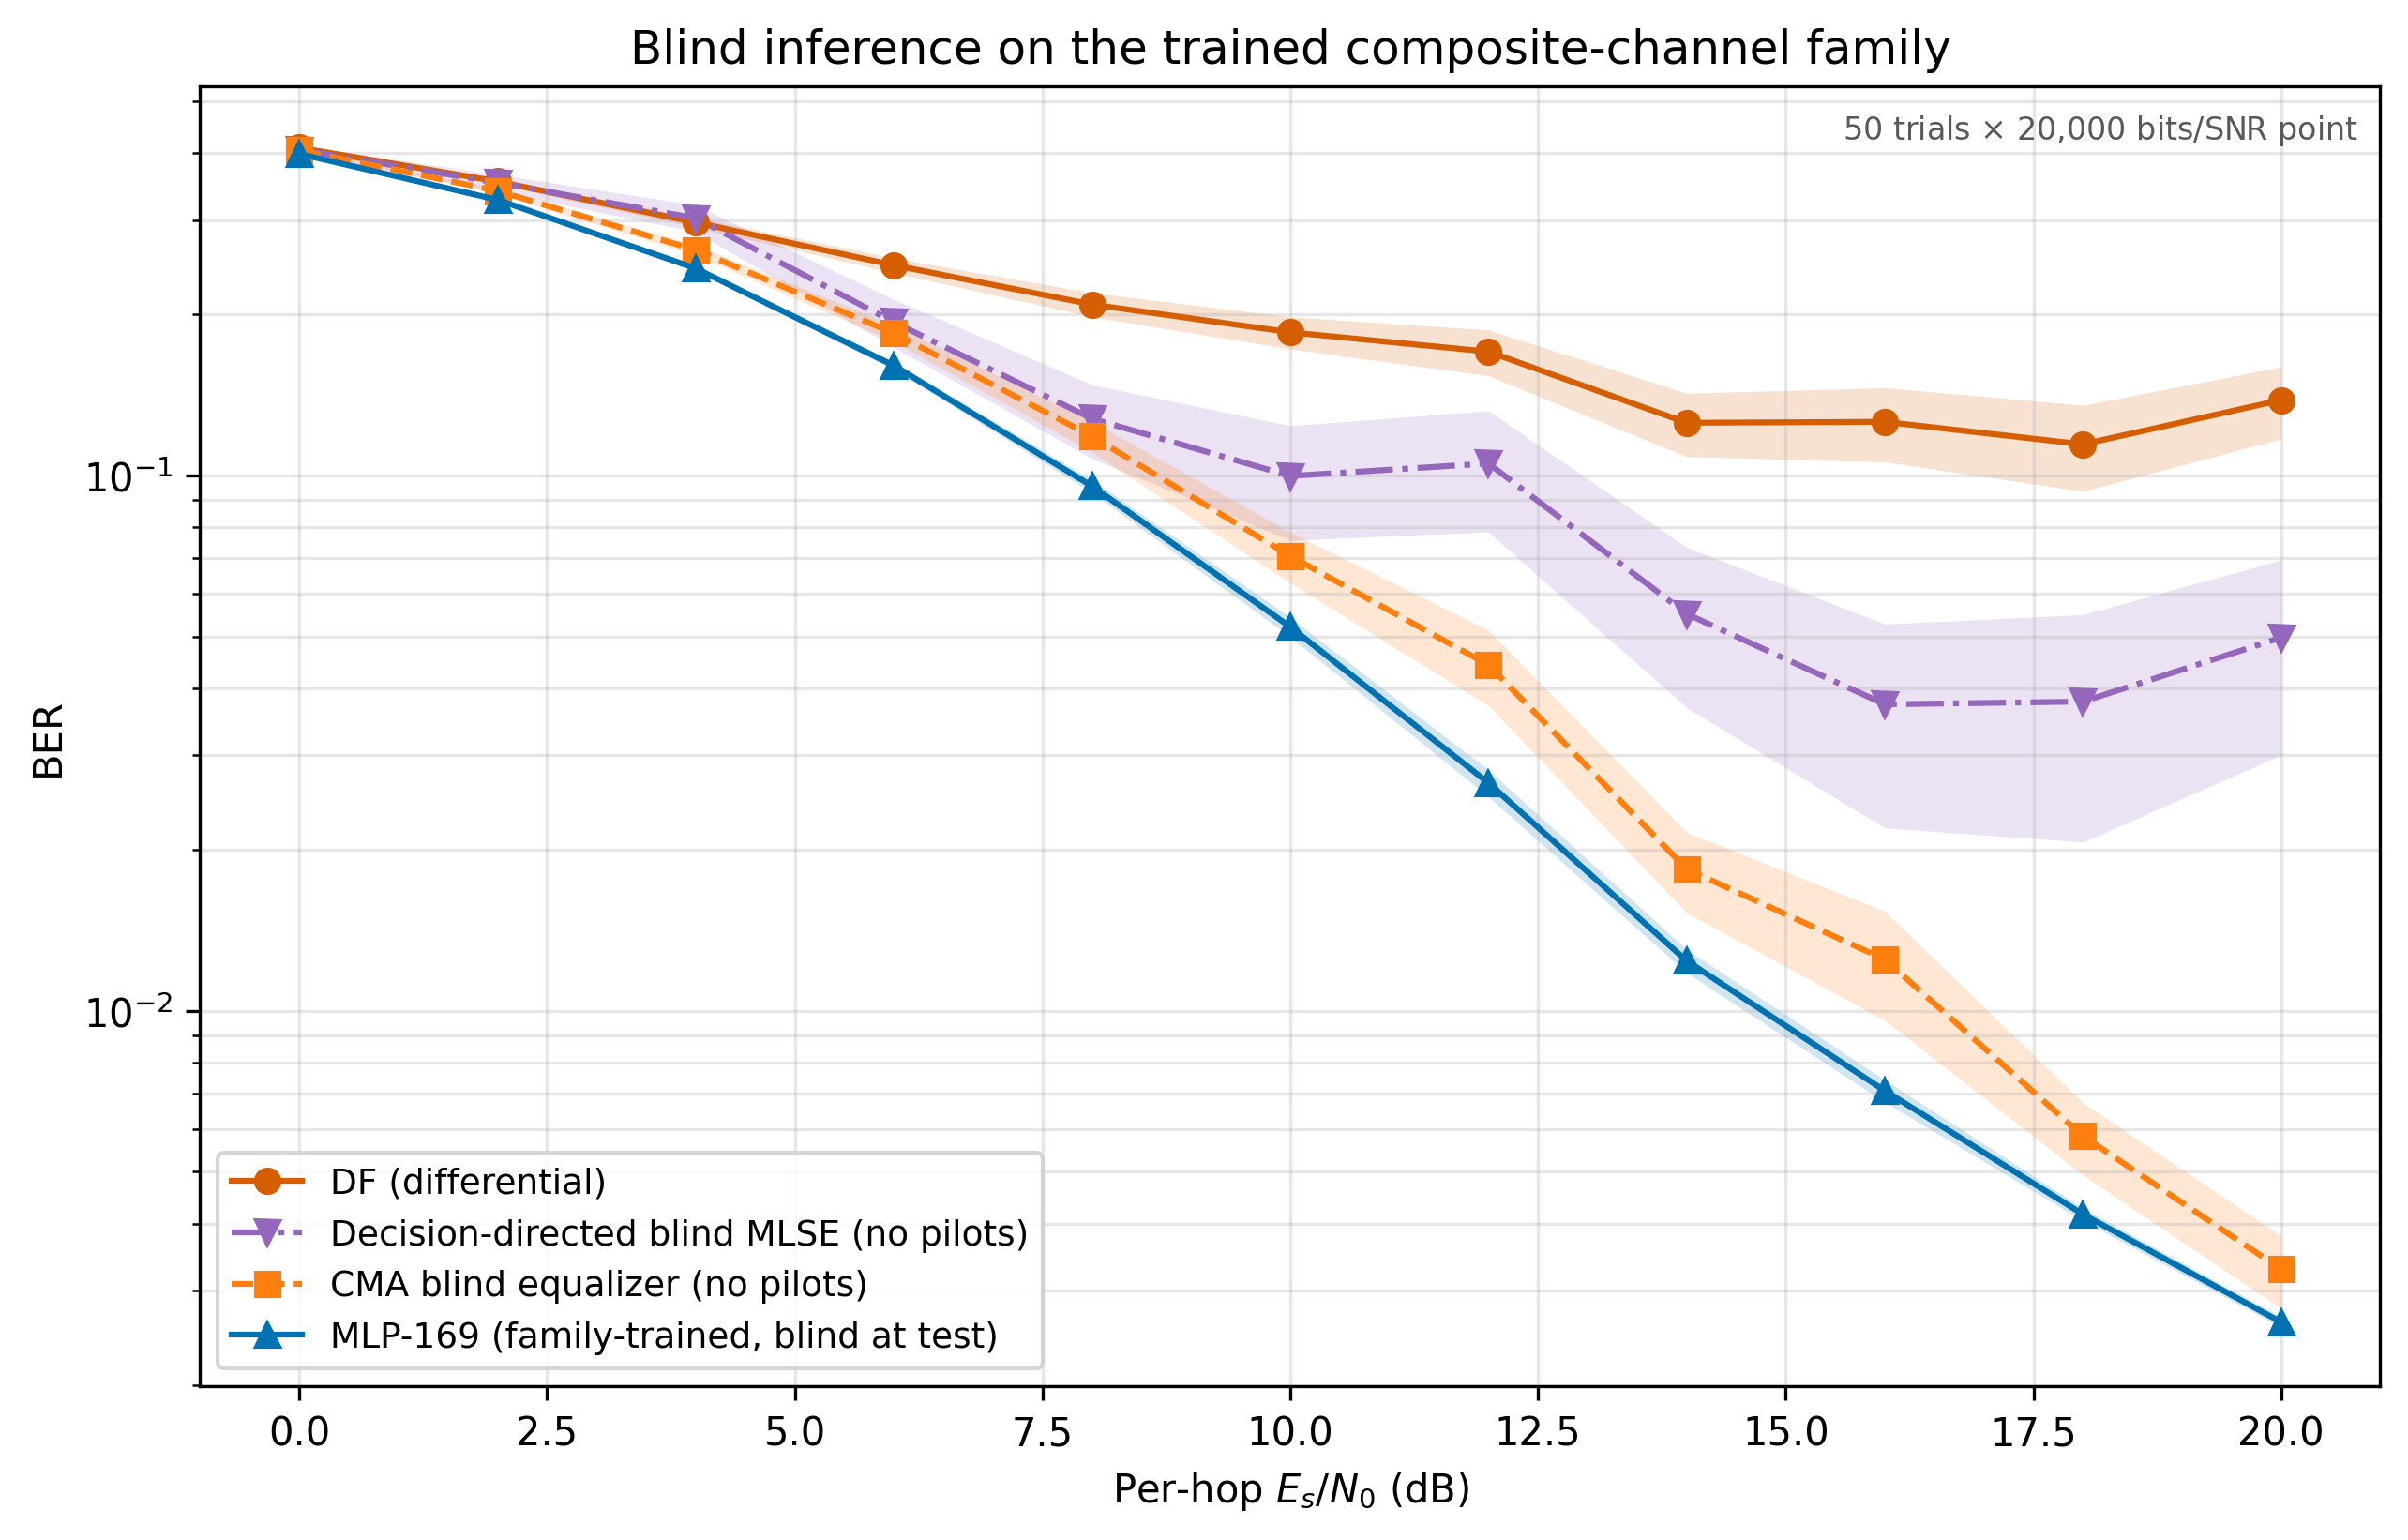
\includegraphics[width=0.82\linewidth,height=0.32\textheight,keepaspectratio]{results/e6_blind.png}}
\caption[Blind composite channel]{No pilots or per-block CSI; fresh realizations from the training family. The evaluated CMA and MLP means are close, while decision-directed MLSE has a non-monotonic high-SNR tail. Historical bands are descriptive; the neural training hierarchy prevents treating all pooled trials as independent confidence evidence. The MLP avoids test-time adaptation but uses family knowledge acquired in training. No claim against all blind equalizers is made}\label{fig:figE6blind}
\end{figure}

\subsection{A Low-Complexity Linear Baseline: MMSE Equalization}\label{sec:mmse-baseline}

The comparisons above set the learned relay against two classical relays, and neither is matched to it in cost. Symbol-wise DF is memoryless and cannot undo intersymbol interference at any transmit power, so outperforming it establishes only that the relay uses its window. Viterbi MLSE is the optimal sequence detector but costs $O(M^{L})$ per symbol in the channel memory, which is precisely the expense Section~\ref{sec:complexity-viterbi-mlp} invokes on the learned relay's behalf. The case between them was not tested: an $N$-tap MMSE linear equalizer is a natural low-complexity remedy an engineer might reach for before a trellis. If it recovered most of what the learned relay recovers, the contribution of Chapter~\ref{sec:unknown-channels} would be a narrower claim about a nonlinearity rather than about learned processing.

It does not. Table~\ref{tbl:mmse-baseline} gives the equalizer's SNR penalty against MLSE for equalizer lengths from 3 to 11 taps, measured on the same two-hop chains, with the exact channel taps supplied and the weights redesigned at every SNR point --- the same genie CSI granted to MLSE, and a longer window than the learned relay is given.

\begin{table}[htbp]
\centering
\caption[MMSE linear equalization against MLSE]{SNR penalty against Viterbi MLSE for an MMSE linear equalizer of $N$ taps, with the best learned relay on the same channel for comparison. Negative values beat MLSE. The reader should observe that the learned relay leads the equalizer by $1.8$ to $2.4$~dB on every channel, despite the equalizer being given exact channel knowledge, per-SNR weight redesign, and up to $11$ taps against the relay's window of $7$}\label{tbl:mmse-baseline}
\begin{tabular}{lrrrrr}
\toprule
Channel & 3 taps & 5 taps & 7 taps & 11 taps & Learned relay \\
\midrule
ISI (BPSK)      & $+6.58$ & $+4.40$ & $+4.23$ & $+4.04$ & $\mathbf{+1.67}$ \\
ISI (QPSK)      & $+7.81$ & $+9.11$ & $+5.02$ & $+4.84$ & $\mathbf{+3.03}$ \\
Composite       & $-0.33$ & $-0.37$ & $-0.37$ & $-0.44$ & $\mathbf{-2.26}$ \\
\bottomrule
\end{tabular}
\end{table}

The learned relay leads the tested linear-MMSE equalizers in the reported required-SNR metric. This is not a comparison against every cost-matched classical method; decision-feedback and reduced-state detectors were not evaluated. The MMSE decreases with filter length, as expected for nested linear estimators. BER and interpolated SNR penalties need not decrease with MSE, however. Consequently the non-monotonic QPSK penalty cannot be dismissed as an interpolation artifact without an additional check. The four-dB sampling grid is a further limitation on the precision of these penalties.

\subsection{Does a Sequence Architecture Help Where a Window Does?}\label{sec:sequence-on-memory}

Chapter~\ref{sec:experiments} finds that Transformer, Mamba-S6 and Mamba-2 buy nothing over a feedforward relay on the canonical channel, and attributes this to the channel rather than to the architectures: a memoryless channel offers no temporal structure for their inductive bias to exploit. That is a prediction about what would happen given such structure, and until now it was untested here, no sequence model having been evaluated anywhere in this chapter. The minimum-size study sharpens the prediction, finding the relay's \emph{window} to be the binding resource on channels with memory, worth $8$ to $11$~dB between window~1 and window~7 while width and depth buy almost nothing. A window is a blunt way of granting a feedforward network temporal context; sequence models are built for it.

The prediction fails. Table~\ref{tbl:seq-on-memory} compares the four architectures at an equal budget of approximately $3{,}000$ parameters, each trained on the channel under test rather than on a memoryless surrogate, with identical hyperparameters and three initializations apiece.

\begin{table}[htbp]
\centering
\caption[Sequence architectures on channels with memory]{SNR penalty against Viterbi MLSE at an equal budget of $\approx$3{,}000 parameters, with the across-initialization spread in brackets. Each entry is the \emph{best} of three initializations, not their mean, so the values are optimistic by construction and the comparison between architectures is only as sound as the bracketed spreads make it; the two Mamba variants' spreads here are wide enough that their ordering against each other should not be read as resolved. Negative values beat MLSE. The reader should observe that the feedforward relay leads every sequence architecture on every channel, and that the two Mamba variants (the most reproducible architectures measured on the canonical channel, at $0.019$ and $0.041$~dB) become the least reproducible here}\label{tbl:seq-on-memory}
\begin{tabular}{lrrrr}
\toprule
Channel & MLP-3K & Transformer-3K & Mamba-S6-3K & Mamba2-3K \\
\midrule
ISI (BPSK) & $\mathbf{+1.97}$ (0.39) & $+3.52$ (0.33) & $+4.30$ (1.15) & $+4.55$ (0.14) \\
ISI (QPSK) & $\mathbf{+2.58}$ (0.07) & $+5.96$ (0.45) & $+5.72$ (1.33) & $+4.69$ (2.12) \\
Composite  & $\mathbf{-2.08}$ (0.03) & $-1.76$ (0.03) & $-1.56$ (0.08) & $-1.60$ (0.06) \\
\bottomrule
\end{tabular}
\end{table}

For this equal-budget, shared-hyperparameter protocol, the feedforward relay has the best reported initialization on all three channels, by $1.55$ and $2.11$~dB on the two ISI cases and $0.32$~dB on the composite. Its observed training times are $35$--$66$~seconds per initialization versus $217$--$609$ for the sequence models. These results favor the tested windowed implementation; they do not establish that channel memory never benefits a tuned sequence architecture.

A second observation was not anticipated. The sequence models' reproducibility inverts. On the canonical channel Mamba-2 and Mamba-S6 are the two most stable architectures measured across initializations; on the complex ISI channel the same architectures spread by more than a decibel (bracketed spreads in Table~\ref{tbl:seq-on-memory}), while the feedforward relay stays inside $0.07$~dB throughout. They are worse on channels with memory, and substantially less predictable there, which compounds the case against them for this task.

One limitation is carried. All four architectures receive identical hyperparameters, matching the equal-budget protocol of Section~\ref{sec:parameter-normalization-complexity-trade-off}; no per-architecture tuning was attempted, and a tuned sequence model might close part of the gap.

\section{The Cost Side: Decision Delay and Arithmetic}\label{sec:complexity-viterbi-mlp}

The cost comparison distinguishes nominal arithmetic from measured implementation time. The BER tradeoff is configuration-dependent, and is not uniformly small, particularly in the QPSK study.

\textbf{Per-symbol cost and scaling.} MLSE maintains $M^{L-1}$ trellis states for a constellation of size $M$ and channel length $L$ (memory $L-1$), performing an add--compare--select over $M^{L}$ branch transitions per symbol; its cost therefore grows \emph{exponentially} in channel memory for fixed $M$, and polynomially in $M$ for fixed $L$. The 170-parameter MLP performs one fixed forward pass, about $330$ floating-point operations per symbol. That figure is a constant of the \emph{deployed} architecture, not a quantity independent of the channel: the input window has to span the memory, so its length grows with $L$, and the output dimension grows with the constellation, from a single real output at $M=2$ to the $193$-parameter QPSK relay used earlier in this chapter, and further still for denser constellations. Once those are fixed, the per-symbol cost is the same for every symbol and every channel realization, which is the property the comparison below relies on. The contrast with MLSE is therefore one of \emph{growth rate}, not of a constant against a variable: the network's cost rises roughly linearly in window length and output dimension, the trellis count is $M^{L}$.

For the studied BPSK three-tap channel, the nominal Viterbi count is about $64$ operations per symbol, below the MLP's approximately $330$ FLOPs (excluding activation-function cost). Full-state trellis counts grow rapidly for larger $M$ and $L$. A fixed network's arithmetic does not depend on the channel realization, but maintaining accuracy as channel complexity increases may require changing its window, width, or output dimension. Extrapolated operation counts for untested architectures are not evidence of retained BER or hardware speedup. Reduced-state sequence detection \cite{EyuboqluQureshi1988RSSE} and decision-feedback methods are unmeasured alternatives.

\begin{figure}[htbp]
\centering
\begin{minipage}[t]{0.49\linewidth}\centering
  \includegraphics[width=\linewidth]{results/e6_per_symbol_cost_vs_modulation_memory.png}
\end{minipage}\hfill
\begin{minipage}[t]{0.49\linewidth}\centering
  \includegraphics[width=\linewidth]{results/e6_right_clean.png}
\end{minipage}
\caption[Complexity: per-symbol cost and measured inference time]{Complexity of Viterbi MLSE against the 170-parameter MLP. \textbf{(a)} Per-symbol computational cost versus modulation order $M$ and channel memory $L$: Viterbi grows as $M^{L}$ (intractable by $M{=}16,L{=}5$), while the network grows only linearly in window length and output dimension ($\sim$330 flops for the deployed BPSK, $L{=}3$ relay). On the small studied channel (BPSK, $L{=}3$) Viterbi is actually cheaper; the MLP wins on \emph{scaling}, not on the small case. \textbf{(b)} Measured inference time for BPSK with $L=3$: the MLP is $30$--$90\times$ faster as a vectorized matmul versus Viterbi's interpreted sequential trellis scan}
\label{fig:figE6complexity}
\end{figure}

\textbf{Measured inference time.} For BPSK with $L=3$, the vectorized NumPy MLP is $30$--$90\times$ faster than the interpreted Python Viterbi implementation on the measured workload, despite Viterbi's lower nominal operation count. This includes implementation overhead. Optimized kernels and target-hardware throughput were not measured; no universal latency or hardware advantage is inferred.

\subsection{A Channel with Memory Under a Latency Constraint}\label{sec:joint-latency-memory}

The accounting above and the ladder that precedes it answer different questions and never meet. The ladder asks which detector is more accurate on a channel with memory, imposing no budget; this section's opening asks what each detector costs, without reference to a channel. What a deployment actually faces is both at once, and the two constraints do not have to bind in the same place. This subsection measures the intersection directly, and includes block DF, which the ladder omits: of the classical options it is the one whose cost is structural rather than arithmetic, so it is exactly the case the ladder's accuracy-only comparison cannot price.

Every scheme is placed inside one identical coded system so that the comparison is between relays and nothing else: a rate-$1/2$, $K=3$ convolutional code on QPSK, $200$ information bits per frame ($202$ symbols after tail), with soft Viterbi decoding of the code at the \emph{destination}. All schemes therefore deliver an information BER at the same information rate. Hop~1 carries the unknown $L$-tap ISI response ($h_k = 0.7^k$, unit-energy normalized) plus complex AWGN and hop~2 is AWGN; $150$ frames per trial and three seeds per point.

Each relay is then labelled with the structural decision delay it forces, in symbols: zero for AF and symbol-wise DF; $\lfloor W/2 \rfloor$ for a relay of window $W$, which must wait for the later half of its own window; $D$ for an MLSE with traceback depth $D$; and the full frame, $202$ symbols, for block DF, which cannot begin until the last symbol of a codeword has arrived.

\paragraph{No latency separation was resolved on the tested short-memory channel.} Table~\ref{tbl:joint-latency} gives the result at $L=3$. The BER at $12$~dB is unchanged at the reported precision from traceback depths $D=2$ through $D=15$. This finite-budget observation does not prove that all survivor paths merge by three symbols or that full-asymptotic accuracy is reached. Among the tested settings, MLSE at $D=2$ has less delay than the window-11 relay's five symbols and lower measured BER. Block DF spends $202$ symbols without a resolved accuracy gain in this experiment; with an equalizer it reproduces the reported MLSE value but adds frame buffering.

\begin{table}[htbp]
\centering
\caption[Relay cost and accuracy under a latency constraint]{Coded information BER at $12$~dB on the three-tap channel, against the structural decision delay each relay forces and its arithmetic per symbol. Mean of three seeds. No BER difference among the tested MLSE traceback depths is resolved at the reported precision; this is not an equivalence or survivor-merger test}\label{tbl:joint-latency}
\begin{tabular}{lrrr}
\toprule
Relay & Delay (symbols) & MACs/symbol & BER at $12$~dB \\
\midrule
AF                    & $0$   & $2$   & $0.0609$ \\
DF-hard (symbol-wise) & $0$   & $0$   & $0.3027$ \\
MLP $W=5$             & $2$   & $112$ & $0.0010$ \\
MLP $W=11$            & $5$   & $208$ & $0.000189$ \\
MLP $W=21$            & $10$  & $368$ & $0.000278$ \\
MLSE $D=2$            & $2$   & $128$ & $\mathbf{0.000033}$ \\
MLSE $D=3$            & $3$   & $128$ & $\mathbf{0.000033}$ \\
MLSE $D=15$           & $15$  & $128$ & $\mathbf{0.000033}$ \\
block DF              & $202$ & $16$  & $0.0411$ \\
block DF $+$ MLSE     & $205$ & $144$ & $0.000033$ \\
\bottomrule
\end{tabular}
\end{table}

The symbol-wise relays confirm the chapter's Layer~2 finding inside the coded chain: AF and hard DF do not merely lose, they fail, DF's BER \emph{rising} with SNR from $0.2913$ at $8$~dB to $0.4253$ at $20$~dB as the interference rather than the noise comes to dominate its decisions.

\paragraph{The cost convention.} Counts below are multiply--accumulates per transmitted symbol, stated here so they can be checked. Additions and comparisons carrying no multiply are excluded; they dominate the trellis search, so the comparison is conservative against this thesis's own conclusion. MLSE has $M^{L-1}$ states and $M$ branches from each, so $M^{L}$ branch metrics per symbol; with the expected observation precomputed each is $|y-c|^{2}$ on a complex difference, two real multiplies, giving $2M^{L}$ (its further $M^{L}$ additions and $M^{L-1}(M-1)$ comparisons are not counted). The relay's $2W$-value input window, the $I$ and $Q$ streams, into $H$ hidden units is $2WH$, and the four-class head $4H$, giving $2WH+4H$; biases are additions and the activations transcendental, so neither is counted.

\paragraph{Arithmetic at a fixed architecture.} With hidden width $H$ fixed, increasing the input window $W$ increases the stated network count linearly, whereas full-state MLSE grows exponentially in tap count $L$ at fixed constellation size $M$. No experiment establishes that fixed $H$ or a particular rule $W=O(L)$ preserves accuracy for arbitrary longer channels. Equating these counts gives an arithmetic crossover, not a universal performance boundary:
\begin{equation}
L^{\star} = \log_{M}\!\left(\frac{2WH + 4H}{2}\right) = 3.35 \text{ taps (MAC-count crossover)}
\label{eq:mac-crossover}
\end{equation}
for $W=11$, $H=8$ and $M=4$ ($2.90$ taps at $W=5$, $3.76$ at $W=21$). At three taps, MLSE's stated count is 128 versus the relay's 208; at seven taps the counts are 32{,}768 and 208. Table~\ref{tbl:joint-memory} reports measured BER separately. The crossover does not assert equal accuracy or a processor-independent speedup.

\begin{table}[htbp]
\centering
\caption[Cost and accuracy against channel memory]{Coded information BER at 12~dB and per-symbol arithmetic. MLSE has genie CSI and traceback $5L$; the 220-parameter window-11 relay is fixed. Measurements at $L=3,5,7$ use 1.5M information bits and five seeds; rows $L=4,6$ contain arithmetic only. Bracketed nominal 95\% Wilson intervals inherit the adjacent BER exponent; coverage under coded error correlations is not established. MLSE has lower measured BER throughout}\label{tbl:joint-memory}
\begin{tabular}{@{}p{0.04\linewidth}p{0.12\linewidth}p{0.14\linewidth}p{0.10\linewidth}p{0.23\linewidth}p{0.22\linewidth}@{}}
\toprule
$L$ & MLSE states & MLSE MACs & Relay MACs & MLSE BER (nominal CI) & Relay BER (nominal CI) \\
\midrule
$3$ & $16$      & $128$      & $208$ & $3.20\times10^{-5}$ \newline [2.41, 4.24] & $2.36\times10^{-4}$ \newline [2.13, 2.62] \\
$4$ & $64$      & $512$      & $208$ & ---                                     & ---                                     \\
$5$ & $256$     & $2{,}048$  & $208$ & $4.20\times10^{-5}$ \newline [3.28, 5.37] & $1.96\times10^{-4}$ \newline [1.75, 2.20] \\
$6$ & $1{,}024$ & $8{,}192$  & $208$ & ---                                     & ---                                     \\
$7$ & $4{,}096$ & $32{,}768$ & $208$ & $2.47\times10^{-5}$ \newline [1.79, 3.40] & $1.91\times10^{-4}$ \newline [1.70, 2.14] \\
\bottomrule
\end{tabular}
\end{table}

In the separately measured three-, five-, and seven-tap settings, the fixed architecture uses $208$ MACs per symbol. Its BER ranges from $1.91\times10^{-4}$ to $2.36\times10^{-4}$; overlapping intervals do not establish constant error or equivalence. The MLSE arithmetic count increases by a factor of $256$, while its measured BER advantage remains configuration-dependent. Under this counting convention, the fixed MLP crosses full-state MLSE in multiplication count between three and five taps. This is not a universal threshold or a guarantee of accuracy beyond the evaluated channels.

Two limits are worth recording. The threshold is a statement about \emph{arithmetic}, not about accuracy: above $L^{\star}$ MLSE remains the more accurate detector wherever it can be afforded, and the learned relay's case rests on it becoming unaffordable rather than on it becoming wrong. And the three-tap channel used throughout this chapter sits \emph{below} $L^{\star}$, so this chapter's earlier results should be read as establishing the failure of the memoryless relays on channels with memory, which they do, and not as a cost argument against MLSE, which at $L=3$ they cannot support.

Taken together, the studies show benefits of the tested learned relays over specified mismatched or memoryless comparators, with limitations from training-family dependence, finite budgets, and untested classical alternatives. They do not overturn the matched memoryless controls or establish a general superiority of learned relaying.
